\lecture{Métodos \textbf{Formais} de Desenvolvimento de Sistemas}{formal}

\frame{\title{\insertlecture}\maketitle}

\begin{frame}{Referência}
  \begin{thebibliography}{10}
    \beamertemplatebookbibitems
  \bibitem[Barret, 2008]{fox2008}
    Clark Barret.
    \newblock Intro to Formal Methods.
    \newblock \href{https://cs.nyu.edu/courses/spring08/V22.0474-001/syllabus.html}{Software Engineering syllabus}.
    \newblock New York University.
  \end{thebibliography}  
\end{frame}

\begin{frame}{Therac-25}
  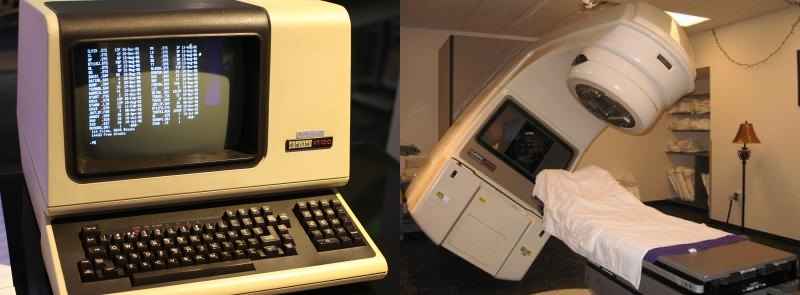
\includegraphics[scale=.5]{therac25.png}
  \fonte{https://notiforo.com/foros/viewtopic.php?t=20164}\bigskip
  
  \begin{itemize}
  \item Entre 1985 e 1987, pelo menos 6 overdoses foram administradas.
  \item Todas as vítimas ficaram com sequelas, 3 morreram.
  \end{itemize}\bigskip

  \href{https://bit.ly/36DJCzi}{Mais detalhes}
  
\end{frame}

\begin{frame}{Ariane 5}\small

  \begin{center}
  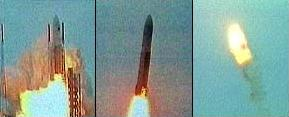
\includegraphics[scale=0.8]{ariane5.png}
  \fonte{\href{https://itsfoss.com/a-floating-point-error-that-caused-a-damage-worth-half-a-billion}
            {https://itsfoss.com/a-floating-point-error-that-caused-a-damage-worth-half-a-billion}}\bigskip
\end{center}

\only<1>{
  No dia \textbf{4 de junho de 1996}, 40 segundos após o lançamento,
  após uma década de esforço da Agência Espacial Europeia e ao custo
  de \$500M, o foguete \alert{Ariane 5} explode devido a um
  \alert{bug} de conversão de \alert{ponto flutuante} no software de
  controle.
}

\only<2-6>{\alert{O que aconteceu?}}

\only<3>{Um número de 64 bits de ponto flutuante relacionado à
  velocidade horizontal do foguete com respeito à plataforma era
  convertido a um inteiro com sinal de 16 bits.}

\only<4>{Quando o número atingiu um valor maior que 32.767, o maior
  valor armazenável em um inteiro com sinal, a conversão
  \alert{falhou}.}

\only<5>{Para piorar a situação o software disparou um sistema de
  diagnóstico que despejou os dados de depuração em uma área de
  memória usada para guiar os motores do foguete.}

\only<6>{Ao mesmo tempo, o controle foi transferido para o computador
  \textit{backup} que tinha os mesmos dados!!!. Isto foi
  mal-interpretado como uma forte necessidade de ação corretiva,
  levando os giros dos motores aos seus limites.}

\begin{center}
\only<7>{\href{https://youtu.be/gp_D8r-2hwk?t=50}{Assistir}}
\end{center}

\end{frame}


\begin{frame}{Mars Climate Orbiter 2}\small
\begin{center}
  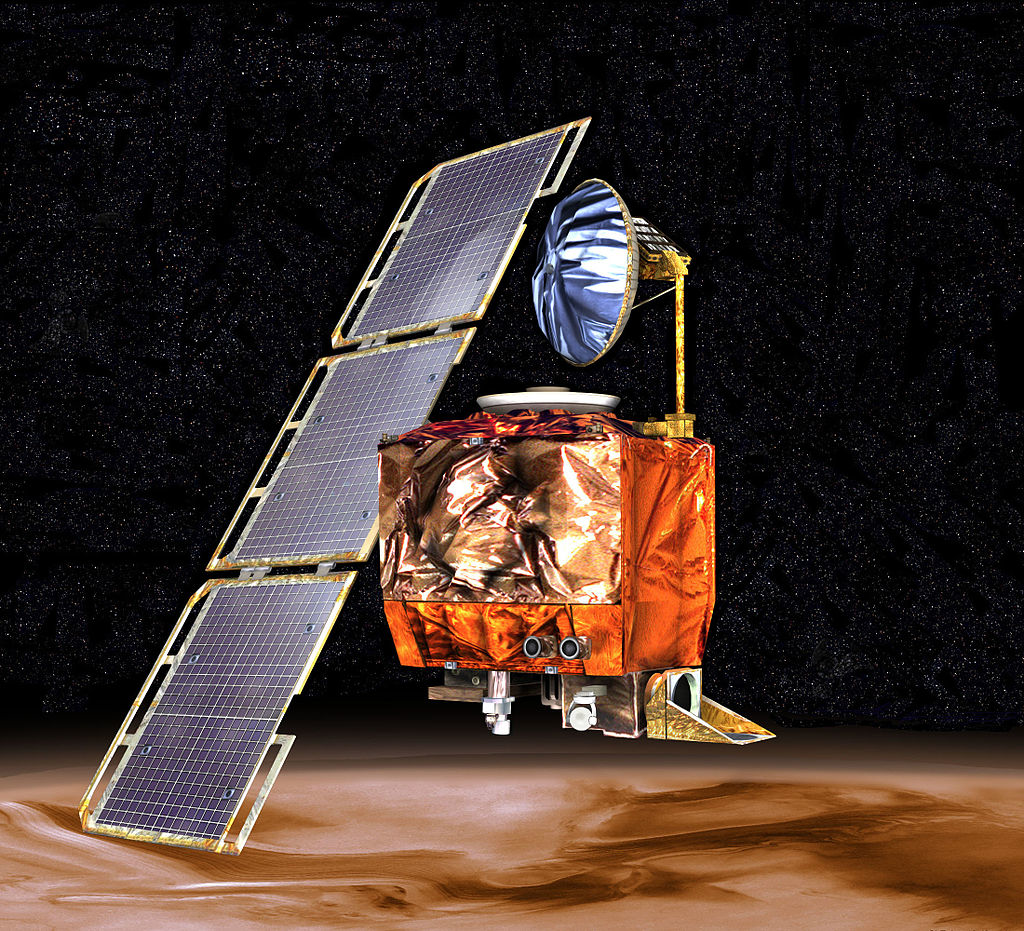
\includegraphics[scale=0.15]{marsorbiter2.png}
\end{center}

\only<1>{Lançada em 11 de dezembro de 1998 para estudar o clima e a
  atmosfera de Marte, bem como as mudanças em sua superfície.}

\only<2>{Porém, em 23 de setembro de 1999, a comunicação com a
  espaçonave é perdida durante à inserção orbital devido a um
  \alert{erro de conversão de unidades, o uso de lbf.s ao invés N.s,}
  no software de controle base.}

\only<3>{A NASA havia investido \$235M na espaçonave.}
  
\end{frame}


\begin{frame}{Variação de complexidade}\small

  \begin{columns}
    \begin{column}{.5\textwidth}
      \begin{center}
        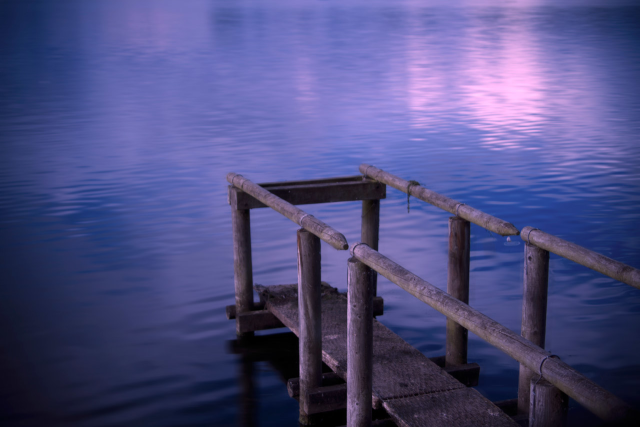
\includegraphics[scale=0.2]{simplebridge.png}
      \end{center}
    \end{column}

    \begin{column}{.5\textwidth}
      \begin{center}
        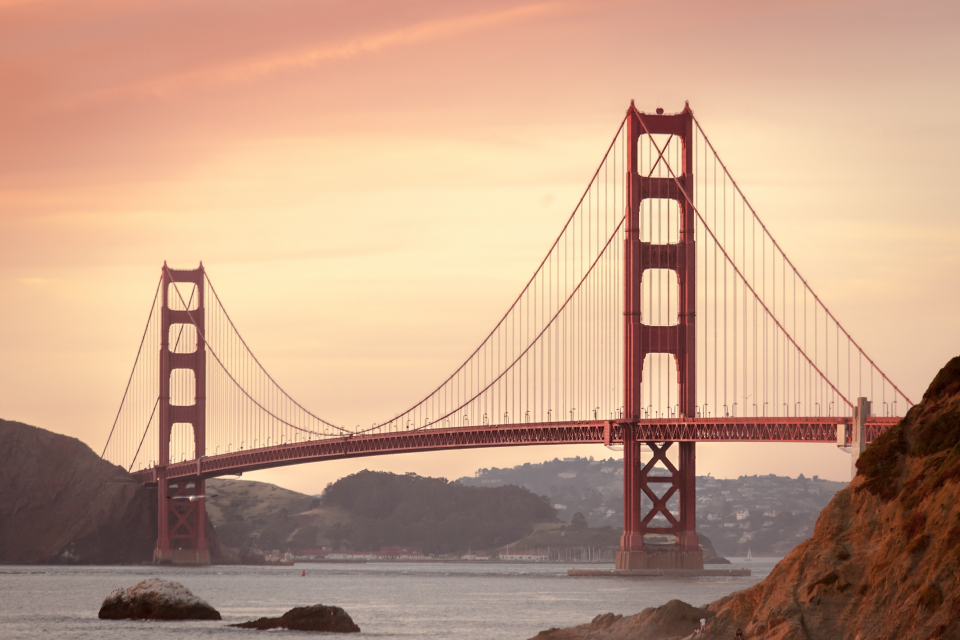
\includegraphics[scale=0.15]{complexbridge.png}        
      \end{center}
    \end{column}
  \end{columns}

  \begin{itemize}
  \item<2-> Alguns erros são muito súbitos ou críticos.
  \item<3-> Especialmente em sistemas concorrente/distribuídos.
  \end{itemize}
  
\end{frame}

\begin{frame}{Perguntas para se pensar}

  \begin{itemize}
  \item<1-> Quando construímos uma ponte ou prédio, não esperamos que eles caiam ou sejam
    reconstruídos duas vezes por semana. Por quê sistemas são menos confiáveis que prédios
    ou pontes?
  \item<2-> Você tem os conhecimentos e habilidades necessárias para
    criar software confiável?
  \item<3-> O que você aprendeu neste curso que pode ajudá-lo com
    relação à pergunta anterior?
  \item<4-> Quais são as ferramentas ou técnicas que você acha que os futuros
    engenheiros de software irão usar para criar sistemas mais confiáveis?
  \end{itemize}
    
\end{frame}


\begin{frame}{Métodos Formais}

  \alert{Como pensar a respeito dos sistemas?}

  \only<2->{Como um cientista! +500 anos de testes com sucesso!}

  \only<3->{A ciência faz \alert{modelos matemáticos} da realidade.}

  \only<4->{Permite clareza de pensamento durante a escrita da especificação.}
  
\end{frame}

\begin{frame}{Classes de Métodos Formais}\footnotesize
  \begin{block}<1-6>{Verificação Formal}
    \begin{itemize}
    \item<2,6> O sistema é descrito em alguma linguagem de especificação;
    \item<3,6> Todos os estados possíveis de serem \alert{alcançados} são testados
      usando um grafo;
    \item<4,6> Uma \alert{desvantagem} é que sistemas muito grandes podem possuir uma
      quantidade excessiva de estados;
    \item<5,6> Porém, esta desvantagem pode ser contornada pela decomposição do sistema
      ou seleção aleatória de apenas alguns estados.
    \end{itemize}
    \end{block}

    \begin{block}<7>{Prova de Teoremas}
      \begin{itemize}
      \item Um sistema automatizado de prova de teoremas é utlizada para
        checar as propriedades do sistema. Isto envolve decodificar os algoritmos
        do sistema para a linguagem do sistema de prova.
      \end{itemize}
  \end{block}
  
\end{frame}


\begin{frame}{(algumas) Ferramentas}\small
  \begin{block}{Verificação formal}
    \begin{description}
    \item<1,5>[\href{http://spinroot.com/spin/whatispin.html}{SPIN}]: Pode
      ser usado para verificação formal de sistemas com múltiplas
      \textit{threads} baseado em lógica Booleana.
    \item<2,5>[\href{http://nusmv.fbk.eu/}{NuSMV}]: Verificador formal de modelo simbólico
      baseado em árvore de decisão binária.
    \item<3,5>[\href{https://lamport.azurewebsites.net/tla/tla.html}{TLA$^+$}]: Construído
      baseado na Lógica Temporal de Ações, permite o uso de prova de Teoremas.
    \item<4,5>[\href{https://www.cs.ox.ac.uk/projects/fdr/}{FDR4}]: Analisa programas
      escritos em CSP$_M$ que combina CSP~(\textit{Communicating Sequential Processes})
      e um linguagem funcional.
    \end{description}
  \end{block}
\end{frame}


%% see also http://www.tptp.org/
\begin{frame}{+(algumas) Ferramentas}\small
\begin{block}{Prova de Teoremas}
    \begin{description}
    \item<1,6>[\href{https://hol-theorem-prover.org/}{HOL}]: Assistente de prova de Teoremas
      interativo que usa a lógica de alta-ordem.
    \item<2,6>[\href{https://isabelle.in.tum.de/}{Isabelle}]: Assistente de prova de Teoremas
      que possui um linguagem matemática para expressão das fórmulas.
    \item<3,6>[\href{https://isabelle.in.tum.de/}{ACL2}]: Possui uma linguagem de programação
      para representação do modelo a ser provado.
    \item<4,6>[\href{http://pvs.csl.sri.com/}{PVS}]: Sistema com linguagem de especificação
      integrada com ferramenta de prova do teorema.
    \item<5,6>[\href{http://cvc4.cs.stanford.edu/web/}{CVC4}]: Especiacilizado em problemas
      de SMT (\text{Satisfiability Modulo Theories}).
    \end{description}
  \end{block}
\end{frame}

\begin{frame}{+(algumas) Ferramentas}\small
\begin{block}{Verificação Formal e Prova de Teoremas}
      \begin{description}
      \item<1,3>[\href{http://why3.lri.fr/}{Why3}]: Plataforma para
        verificação de programas baseada na linguagem {\tt WhyML} e
        que usa ferramentas externas para Provas de Teoremas.
        \item<2,3>[\href{https://lamport.azurewebsites.net/tla/tla.html}{TLA$^+$}]: {\bf Construído
        baseado na Lógica Temporal de Ações, permite o uso de prova de Teoremas.}
      \end{description}
    \end{block}
\end{frame}